\documentclass{standalone}
\usepackage{tikz}
\usetikzlibrary{patterns}

\begin{document}
  \begin{figure}[h]
    \raisebox{-0.5\height}{
      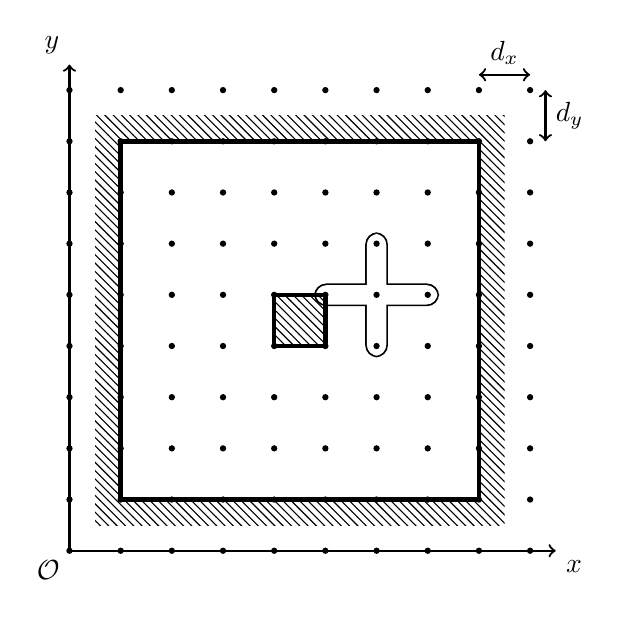
\begin{tikzpicture}[scale=0.65]
        \draw[draw=none,pattern=north west lines] (0.5,0.5) rectangle (8.5,8.5);
        \draw[ultra thick,fill=white] (1,1) rectangle (8,8);

        \draw[thick,rounded corners=4] (4.8,4.8) rectangle (7.2,5.2);
        \draw[thick,rounded corners=4] (5.8,3.8) rectangle (6.2,6.2);
        \draw[draw=none,rounded corners=4,fill=white] (4.81,4.81) rectangle (7.19,5.19);
        \draw[draw=none,rounded corners=4,fill=white] (5.81,3.81) rectangle (6.19,6.19);

        \draw[ultra thick,pattern=north west lines] (4,4) rectangle (5,5);

        \draw[thick,->] (0,0) -- (9.5,0) node[anchor=north west] {$x$};
        \draw[thick,->] (0,0) -- (0,9.5) node[anchor=south east] {$y$};
        \node[anchor=north east] at (0,0) {$\mathcal{O}$};
        \foreach \x in {0, ..., 9} {
          \foreach \y in {0,...,9} {
            \draw[radius=0.05,fill=black] (\x,\y) circle;
          }
        }

        \draw[thick,<->] (8,9.3) -- (9,9.3) node[anchor=south] at (8.5,9.3) {$d_x$};
        \draw[thick,<->] (9.3,8) -- (9.3,9) node[anchor=west] at (9.3,8.5) {$d_y$};
      \end{tikzpicture}
    }
    \hfill
    \raisebox{-0.5\height}{
      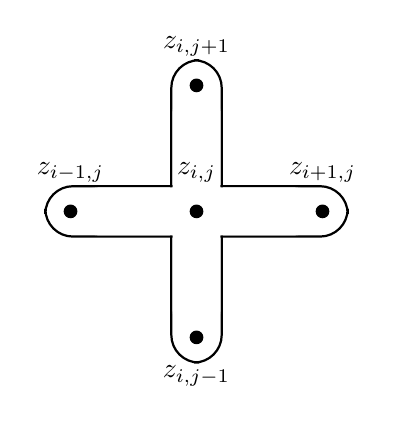
\begin{tikzpicture}[scale=1.6]
        \draw[thick,rounded corners=10] (-0.2,0.8) rectangle (2.2,1.2);
        \draw[thick,rounded corners=10] (0.8,-0.2) rectangle (1.2,2.2);
        \draw[draw=none,rounded corners=10,fill=white] (0,0.81) rectangle (2,1.19);
        \draw[draw=none,rounded corners=10,fill=white] (0.81,0) rectangle (1.19,2);

        \draw[radius=0.05,fill=black] (1,2) circle node[anchor=south] at ++ (0,0.15) {$z_{i,j+1}$};
        \draw[radius=0.05,fill=black] (0,1) circle node[anchor=south] at ++ (0,0.15) {$z_{i-1,j}$};
        \draw[radius=0.05,fill=black] (1,1) circle node[anchor=south] at ++ (0,0.15) {$z_{i,j}$};
        \draw[radius=0.05,fill=black] (2,1) circle node[anchor=south] at ++ (0,0.15) {$z_{i+1,j}$};
        \draw[radius=0.05,fill=black] (1,0) circle node[anchor=north] at ++ (0,-0.15) {$z_{i,j-1}$};
      \end{tikzpicture}
    }
  \end{figure}
\end{document}
